\chapter{Monitoring DLAKaApp}
\label{cha:first_solution}

This chapter applies the extended UME approach from Chapter \ref{cha:concept} to the BestRentalPoC
by extending its story that requires the integration of monitoring. The name of the developed monitoring
software is SPMonitor. The chapter is oriented along the different phases of software development.
First, Section \ref{sec:motivation} extends the story of BestRentalPoC.
Then follow the analysis of SPMonitor in Section \ref{sec:analysis}, the design in Section \ref{sec:design},
and the implementation and deployment in Section \ref{sec:impl_and_deployment}.

\section{Motivation}
\label{sec:motivation}

The development of SPMonitor will be based on the following motivation story.
This extends the story of the BestRentalPoC.

The DrivingLicenseAuthorityKarlsruhe (DLAKa) wants to provide citizens with digital driving licenses,
which can, for example, be used by citizens to prove to a car rental company that they possess a valid driving license.
They hire the company ServiceProvider (SP) to develop and operate the system necessary for issuing and verifying
digital driving licenses. The contract specifies an initial payment for the development of the system
and afterward a yearly fee for the operation of the system.
After receiving the contract from DLAKa, SP starts to design the system
for DLAKa. Because SP has to operate the system on a fixed yearly budget,
they want to monitor the performance of the system to identify parts with excessive resource usage, which
incur additional costs. They identify the memory usage of the system as a technical metric that should be monitored.
This metric will be called MemUse (Memory Usage).
Additionally, \Gls{DLAKa} has asked SP to provide the capability of monitoring business metrics for them.
\Gls{DLAKa} wants to know how many digital driving licenses are being issued. 
This metric will be called NumDDL (Number of Issued Digital Driving Licenses).
To monitor both technical and business metrics, SP designs the ServiceProviderMonitor (SPMonitor) as a part
of the system for \Gls{DLAKa} which will provide all functionality for monitoring the specified metrics.

\section{Analysis}
\label{sec:analysis}

The following section will provide an analysis of SPMonitor based on the motivation above.
Firstly, use cases are derived from the motivation above. These use cases are then used
to derive capabilities and requirements for SPMonitor. This will be followed by defining
the metrics that SPMonitor will collect. Finally, SPMonitor will be analyzed regarding its
integration with DLAKaApp and modifications that might have to be made in DLAKaApp.

\subsection{Use Cases}

Based on the motivation, three use cases for SPMonitor were derived: Inspect Metric, Configure Metric, and Assign Permissions.
The use case Inspect Metric is concerned with the presentation of monitoring data to the users of SPMonitor.
The use case Configure Metric describes how metrics will be added to SPMonitor.
Lastly, the use case Assign Permissions covers the control of access to the collected data.
The relation of these use cases can be seen in Figure \ref{fig:use_case_diagram_spmonitor} as a use case diagram.

\begin{figure}
	\centering
	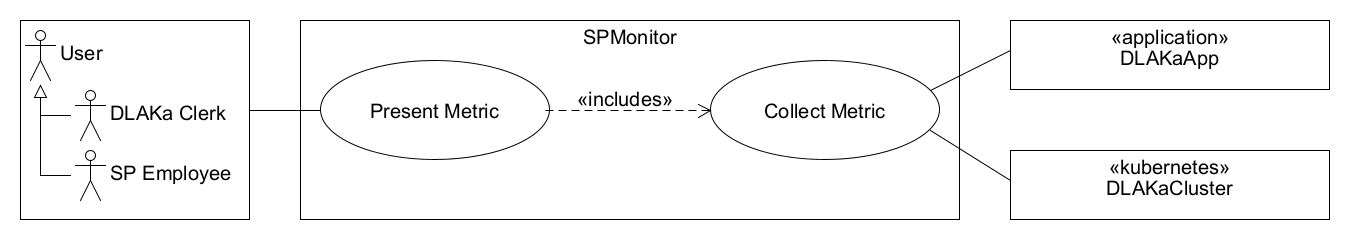
\includegraphics[width=\textwidth]{figures/2.1_use_case_spmonitor.png}
	\caption{Use Case Diagram: SPMonitor}
	\label{fig:use_case_diagram_spmonitor}
\end{figure}

The use case description of the Inspect Metric use case can be seen in Listing \ref{lis:use_case_description_inspect_metric}.
The use case has two primary actors DLAKa Clerk and SP Employee.
Both of these primary actors are a user of SPMonitor who differ in their assigned roles.
A user of SPMonitor can have one of two roles. Firstly, a user could work for DLAKa and thus have the role
DLAKa Clerk. The other possibility is that the user could work for SP and have the role SP Employee.
Due to possible privacy concerns, each user can only have one of these two roles.
Based on their role they will be able to access different dashboards which contain different data.
The preconditions of this use case are that a metric has been configured for collection and that a dashboard
has been set up that the user wants to access. A dashboard presents related monitoring data as a collection of graphs.
After the user selects a dashboard, SPMonitor will retrieve the stored values for the dashboard and display
them in graphs. Alternatively, if the user does not have the permission to access the dashboard,
SPMonitor will not open the dashboard for the user.

\begin{lstlisting}[caption = {Use Case Description: Inspect Metric}, label = {lis:use_case_description_inspect_metric}, style = kit-cm, language=]
Title: Inspect Metric

Primary Actors: DLAKa Clerk, SP Employee

Preconditions:
- SPMonitor has a metric configured
- SPMonitor has a dashboard for the metric configured

Flow:
1. The user opens a dashboard for a metric
2. SPMonitor retrieves all stored values for that metric
3. SPMonitor displays the values to the user in the dashboard

Alternative Flows:
1a. The user does not have the permission to access the dashboard
2a1. The user can not open the dashboard

Information Requirements:
- Values for the metric
\end{lstlisting}

The use case description of the Configure Metric use case can be seen in Listing \ref{lis:use_case_description_configure_metric}.
This use case has one primary actor who works for SP as a developer, called SP Developer.
Additionally, the use case has two secondary actors the DLAKaApp and the DLAKaCluster.
DLAKaApp is the application that is being monitored and DLAKaCluster is a Kubernetes
cluster that represents DLAKaApp's runtime environment.
First SP Developer configures the collection of a metric. This involves setting up
either the DLAKaApp or DLAKaCluster to emit the metric that should be collected
and then setting up SPMonitor to collect that metric. After SPMonitor collects the metric,
SP Developer configures a dashboard for that metric. After the graphs for the dashboard
have been created SP Developer selects which of the two roles DLAKa Clerk or SP Employee
can access the dashboard.

\begin{lstlisting}[caption = {Use Case Description: Configure Metric}, label = {lis:use_case_description_configure_metric}, style = kit-cm, language=]
Title: Configure Metric

Primary Actor: SP Developer
Secondary Actors: DLAKaApp, DLAKaCluster

Flow:
1. SP Developer configures the collection of a metric
2. SP Developer configures a dashboard for the metric
3. SP Developer configures the permissions of the dashboard
\end{lstlisting}

The use case description of the Assign Permissions use case can be seen in Listing \ref{lis:use_case_description_assign_permissions}.
This use case has SP Developer as its primary actor. Before this use case,
SPMonitor must have a registered user. SP Developer assigns this registered user
either the role DLAKa Clerk or SP Employee depending on which organization the user belongs to.

\begin{lstlisting}[caption = {Use Case Description: Assign Permissions}, label = {lis:use_case_description_assign_permissions}, style = kit-cm, language=]
Title: Assign Permissions

Primary Actor: SP Developer

Preconditions:
- SPMonitor has a registered user

Flow:
1. SP Developer assigns a user permission to access a dashboard
\end{lstlisting}

\subsection{Metrics Definition}
The NumDDL metric should represent the number of issued digital driving licenses.
Therefore its value should be incremented each time the DLAKaApp completes the issuing of
a digital driving license. The metric NumDDL will always be an integer.
The metric NumDDL should be presented as a line graph that visualizes the development
of the metric.
The MemUse metric should represent the amount of memory that is currently being used by the
DLAKaApp. For better understandability, the metric should be presented in several forms.
Firstly, the MemUse metric should measure the total amount of memory used by DLAKaApp
and present it as a percentage of a set maximum of usable memory. Additionally,
the MemUse metric should present the same information for each service
of DLAKaApp where each service has an individual maximum of usable memory.
The total maximum usable memory should be the sum of the maximums of the individual services.
These percentage-based values should be represented as gauges.
In addition to the percentage-based values, the MemUse metric should also
display the current total memory usage of DLAKaApp and each service
in megabytes. The current total memory usage of DLAKaApp should be visualized as a line graph.
The memory usage of the services should be presented in a combined line graph.
Both metrics will be represented in separate dashboards.

\subsection{Capabilities and Requirements}

\begin{table}[]
\centering
\begin{tabular}{l}
Requirements \\
\hline
R1: User Interface, Data Source and Data Sink \\
R2: User Accounts and Role-Based Access Control \\
R3: Support Metric Collection from Kubernetes and Golang microservices \\
R4: Support Kubernetes as a Runtime \\
R5: Permissive Licenses \\
\end{tabular}
\caption{Requirements for SPMonitor}
\label{tab:spmonitor_requirements}
\end{table}

From the use cases, the capabilities and requirements for SPMonitor can be derived.
First the capabilities. SPMonitor needs to be able to collect metrics from DLAKaApp and the DLAKaCluster.
These metrics need to be stored. The metrics should be visualized by SPMonitor in pre-configured dashboards.
Users of SPMonitor must be able to access the system with a registered account that is in their name.
SPMonitor also needs to support role-based access control for access to the dashboards.
From the use cases and the capabilities, the requirements for SPMonitor can be derived.
The requirements that have been derived are listed in Table \ref{ref:spmonitor_requirements}.
Based on the use cases SPMonitor requires all three components of a monitoring system: A user interface, a data source
and a data sink. SPMonitor also requires a system through which users can be registered and assigned different role-based
permissions. Because SPMonitor needs to interact with the secondary actors DLAKaApp and the DLAKaCluster,
SPMonitor needs to be able to collect metrics from a microservice implemented in Golang as well as from
a Kubernetes cluster. Due to the scope of this thesis, there are two additional requirements.
First, SPMonitor should be able to run inside the Kubernetes cluster DLAKaCluster.
Second, all tools required by SPMonitor to operate should have a license that allows free usage
and is open source.

\subsection{Integration with DLAKaApp}

% TODO: Check

SPMonitor will need to be integrated with DLAKaApp to function.
The integration with SPMonitor will target two components of the DLAKaApp:
The application microservice DrivingLicenseManagement and the runtime environment, of DLAKaApp, DLAKaCluster.
Firstly, SPMonitor needs to be able to send requests to the application microservice DrivingLicenseManagement.
This microservice will also need to be modified so that it collects the NumDDL metric and can reply
with its value when it receives the corresponding request from SPMonitor.
As a result, the API specification of DrivingLicenseManagement will need to be updated to include
an endpoint for communication with SPMonitor. Additionally, the architecture of DrivingLicenseManagement
needs to be changed to include the necessary components for the collection of the NumDDL metric
and the communication with SPMonitor.
Contrary to the application microservice DrivingLicenseManagement, DLAKaCluster will only
need to be correctly configured during development as Kubernetes already provides functionality
to expose the MemUse metric.

\section{Design}
\label{sec:design}

% TODO: Section intro

\subsection{Abstract SPS Architecture}

% TODO: Check

\begin{figure}[h]
	\centering
	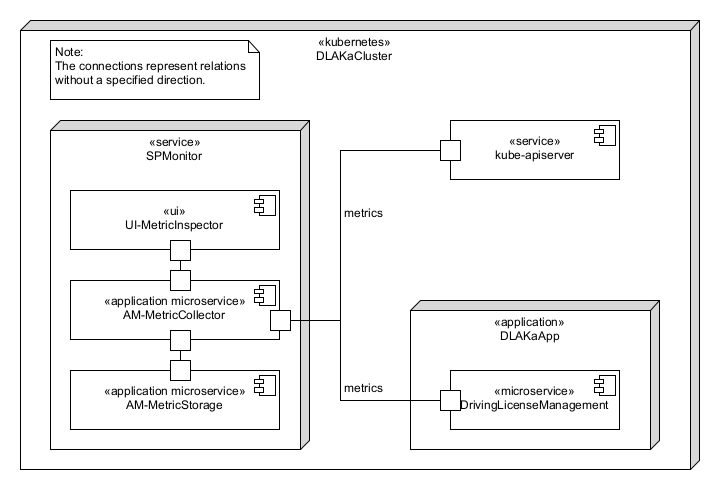
\includegraphics[width=\textwidth]{figures/abstract_sps_spmonitor.png}
	\caption{Abstract SystemPlusSoftware Architecture for SPMonitor}
	\label{fig:abstract_sps_spmonitor}
\end{figure}

Based on the above analysis, an abstract SPS (SystemPlusSoftware) architecture was created for SPMonitor.
The architecture can be seen in Figure \ref{fig:abstract_sps_spmonitor}.
In this architecture, no concrete tools are considered. Instead, only abstract components
and their interactions are visualized.
SPMonitor will consist of two microservices and a user interface.
The user interface provides the functionality of displaying the collected metrics
in dashboards and graphs. The Data Source microservice is responsible for collecting
the metrics from DLAKaApp. It also provides an interface for the user interface
to access the stored values of the metrics. The Data Sink microservice handles the storage
of the metric values and provides an interface to the Data Source for storing and accessing
collected metric values.
The metric NumDDL will be collected from the DLAKaApp microservice DrivingLicenseManagement
and the metric MemUse will be collected from the DLAKaCluster which is a Kubernetes cluster
that provides the runtime of the DLAKaApp.
For the collection of the metrics, both the DLAKaApp and the DLAKaCluster need to provide
an interface through which the Data Source microservice can collect their respective metrics.

\subsection{API Specification}

% TODO: Check

The abstract SPS architecture defined in Figure \ref{fig:abstract_sps_spmonitor} requires
the DLAKaApp to provide two interfaces through which SPMonitor can collect metrics.
The DLAKaCluster running in Kubernetes already provides the required interface 
through an HTTP endpoint at clusterURL/metrics. The application microservice DrivingLicenseManagement
will have to be adapted with a similar endpoint. It will also be hosted on the path /metrics
and export metrics in the same format as Kubernetes does. The actual format of the exported metrics
might have to change later if the data source that will be used requires a different format
but the endpoint will conceptually still be the same. The format used by Kubernetes is the Prometheus
metrics format. In this format, each metric is expressed as three lines of text. The first line
provides information about the meaning of the metric. The second line declares the type of metric.
In the case of NumDDL, this is a counter which is a positive integer that can never decrease.
The last line contains the name of the metric and its value. Optionally, the last line
can also contain a set of labels with assigned values. Labels are not used for the NumDDL metric.
The API specification of the metrics endpoint for DrivingLicenseManagement can be seen in Listing \ref{lis:api_spec_drivinglicensemanagement}
which is written using the OpenAPI standard.

\begin{lstlisting}[caption = {Partial API Specification of Application Microservice DrivingLicenseManagement}, label = {lis:api_spec_drivinglicensemanagement}, style = kit-cm, language=]
openapi: 3.0.0
info:
  title: Partial API of Application Microservice DrivingLicenseManagement
  version: 1.0.0
paths:
  /metrics:
    get:
      responses:
        200:
          description: Success
          content:
            text/plain:
              schema:
                type: string
              examples:
                has_value: 
                  summary: The metric has a value
                  value: |
                    # HELP num_ddl Number of issued digital driving licenses
                    # TYPE num_ddl counter
                    num_ddl 42
                no_value: 
                  summary: The metric has no value
                  value: |
                    # HELP num_ddl Number of issued digital driving licenses
                    # TYPE num_ddl counter
                    num_ddl 0
\end{lstlisting}

The API diagram of the application microservice DrivingLicenseManagement also needs to be adapted
to provide the functionality of exporting metrics on an HTTP endpoint. The API diagram
represents the logical connection between different endpoints in the style of Domain-Driven Design.
% TODO: rewrite to fit diagram shown
% The changes to the diagram consist of two additional entities: The MetricsCollector and the Metric.
% The Metric entity represents a single integer valued metric. Each metric has a name, a current value,
% and an optional list of labels. The value of the metric can be updated or exported which constructs
% a string in the format used by the API Specification in Listing \ref{lis:api_spec_drivinglicensemanagement}.
% The MetricsCollector entity is a collection of Metric entities. While there is only one metric currently,
% this design was chosen as it also extensions in the future. Through the MetricsCollector the value of
% a metric can be updated by DrivingLicenseManagement. For the case of NumDDL, this update happens from
% the createIssuance method which creates digital driving licenses.
% The MetricsCollector also provides a method for exporting all metrics. This returns the combination
% of each metric's representation as a string in the form of an HTTP response.
% The exportAll method is the method that is responsible for handling the metrics endpoint. All other
% added methods just provide the logic needed for exporting the metrics.
% The adapted API diagram can be seen in Figure \ref{fig:api_diagram_drivinglicensemanagement}.

% \begin{figure}[h]
% 	\centering
% 	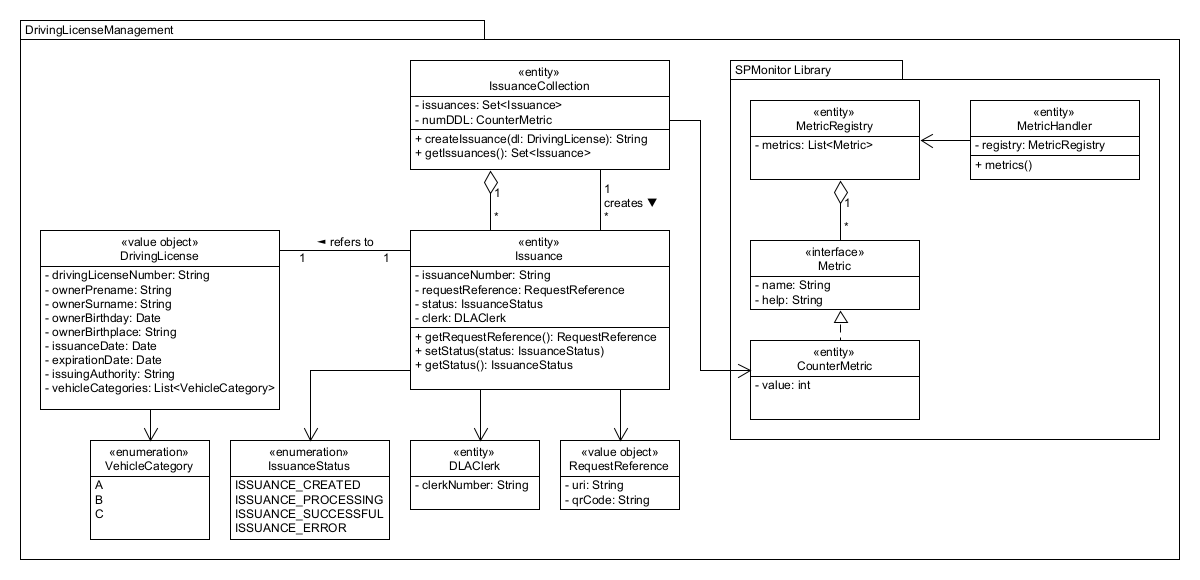
\includegraphics[width=\textwidth]{figures/api_diagram_drivinglicensemanagement.png}
% 	\caption{API Diagram DrivingLicenseManagement}
% 	\label{fig:api_diagram_drivinglicensemanagement}
% \end{figure}

% TODO: Ref Roman for implementation of SPMonitor Client Lib in DLM

\subsection{Tool Selection Based on Capabilities and Requirements}

% TODO: Update to new requirements layout

% As explained in Chapter \ref{cha:technical_foundation}, a monitoring system consists of three parts:
% The Data Source, Data Sink and a tool for visualization.
% The data source is the core of a monitoring system. It is responsible for collecting the monitoring data
% and dictates the needs for the data sink as well as the possibilities for the visualization.
% Because of its central role, the data source will be the first component of the monitoring system that will be chosen
% and the rest of the monitoring system will be chosen to best fit with and support the data source.

% In order for the chosen data source to best fit the needs of SPMonitor, it needs to fulfill some requirements
% which stem from SPMonitor's use cases. The first requirement for the data source is that it should be built
% to support the use cases of SPMonitor. Tools that are built for different purposes but could be used for SPMonitor's
% use cases, will be less preferable than tools that are designed for SPMonitor's use cases.
% Secondly, the data source should be free to use. This requirement mostly stems from the scope of this work
% as a bachelor's thesis without any funding.
% Additionally, the data source needs to be able to collect technical metrics as well as business metrics.
% While technical metrics can be gathered from most cloud environments automatically, business metrics
% require the instrumentation of the source code of the monitored services. Many data sources can in theory
% instrument service but they often use additional tools like OpenTelemetry for this. Because SPMonitor aims
% to be as slim as possible, to reduce complexity, data sources that can instrument services on their own without
% the need for an additional tool, will be preferred over data sources that can not do that.
% Lastly, the data source needs to support two different cloud environments: Kubernetes for the on-premise parts
% of \Gls{DLAKaApp} and Microsoft Azure for the decentralized identity part of DLAKaApp.

% These six requirements for the data source are listed in Table \ref{tab:data_source_requirements}.
% Requirements R2 through R6 are hard requirements, meaning that a data source that does not fulfill them
% will not be chosen. Requirement R1 is a soft requirement that is meant as an orientation and does directly
% lead to the elimination of a data source.

% \begin{table}[]
% \centering
% \begin{tabular}{c|l}
% Key & Requirements \\
% \hline
% R1 & Purpose \\
% R2 & Licensing \\
% R3 & Technical metrics \\
% R4 & Business metrics \\
% R5 & Kubernetes \\
% R6 & Microsoft Azure \\
% \end{tabular}
% \caption{Requirements for the Data Source}
% \label{tab:data_source_requirements}
% \end{table}

% The data sources that will be compared according to the requirements in Table \ref{tab:data_source_requirements} stem
% from the paper \enquote{A Survey on Observability of Distributed Edge {\&} Container-Based Microservices}
% by Usman et al. \cite{UF+22}. The list from that survey was supplemented with one additional entry,
% the TICK (Telegraf, InfluxDB, Chronograf, Kapacitor) stack. Any entries that do not support metrics or are purely research projects were eliminated.
% Lastly, the entry for Kibana was changed to ELK for the ELK (ElasticSearch, LogStash, Kibana) stack.
% The complete overview of all analyzed tools can be seen in Table \ref{tab:data_source_comparison}.

% \begin{table}[]
% \centering
% \begin{tabular}{l|c|c|c|c|c|c}
% Name & R1 & R2 & R3 & R4 & R5 & R6 \\
% \hline
% Apache SkyWalking		 & Performance & Free & \cmark & \cmark & \cmark & \xmark \\
% Cilium					 & Networking & Free & \cmark & \xmark & \cmark & \cmark \\
% Datadog					 & SaaS & Paid & \cmark & \cmark & \cmark & \cmark \\
% Dynatrace				 & PaaS & Paid & \cmark & \xmark & \cmark & \cmark \\
% ELK						 & Searching & Paid & \cmark & \xmark & \cmark & \cmark \\
% Honeycomb				 & Debugging & Paid & \cmark & \cmark & \cmark & \cmark \\
% Instana					 & Incidence Management & Paid & \cmark & \xmark & \cmark & \cmark \\
% Monasca					 & MaaS & Free & \cmark & \xmark & \cmark & \xmark \\
% New Relic				 & PaaS & Paid & \cmark & \cmark & \cmark & \cmark \\
% \rowcolor{lightgray}
% OpenTelemetry			 & Monitoring & Free & \cmark & \cmark & \cmark & \cmark \\
% \rowcolor{lightgray}
% Prometheus				 & Monitoring & Free/Paid & \cmark & \cmark & \cmark & \cmark \\
% Scalyr					 & PaaS & Paid & \cmark & \xmark & \cmark & \xmark \\
% SolarWinds				 & PaaS & Paid & \cmark & \xmark & \cmark & \cmark \\
% Splunk					 & Resilience & Paid & \cmark & \cmark & \cmark & \cmark \\
% Sumo Logic				 & Analytics & Paid & \cmark & \cmark & \cmark & \cmark \\
% \rowcolor{lightgray}
% TICK					 & Time Series Data & Free/Paid & \cmark & \cmark & \cmark & \cmark \\
% \end{tabular}
% \caption{Comparison of data sources}
% \label{tab:data_source_comparison}
% \end{table}

% The three final candidates for use in SPMonitor can be seen highlighted in Table \ref{tab:data_source_comparison}.
% They are OpenTelemetry, Prometheus, and the TICK stack.
% OpenTelemetry is a standalone solution for the collection of metrics. 
% It provides many client libraries to instrument service for business metrics and can integrate
% with most data sinks and visualization tools.
% Prometheus is commonly used in combination with the LGTM (Loki Grafana Tempo Mimir) stack.
% Loki is a service for handling logs, Tempo is responsible for handling traces, Grafana is used for visualization and Mimir provides
% long-term storage for Prometheus. Prometheus itself is responsible for the collection of metrics.
% As this work only considers metrics, the full setup would use Grafana for visualization, Prometheus as the data source, and Mimir
% as the data sink. As Mimir only provides Prometheus with an interface to a storage system and is itself not one, it can be paired with MinIO
% a free-to-use object storage system.
% The TICK stack consists of four different tools: Telegraf, InfluxDB, Chronograf, and Kapacitor.
% Telegraf is responsible for collecting metrics from the monitored services. The collected metrics are then forwarded
% to InfluxDB, the storage component of the stack, and Kapacitor which is responsible for data processing.
% Chronograf provides the interface to visualize and analyze the collected metrics.

% \begin{figure}[h]
% 	\centering
% 	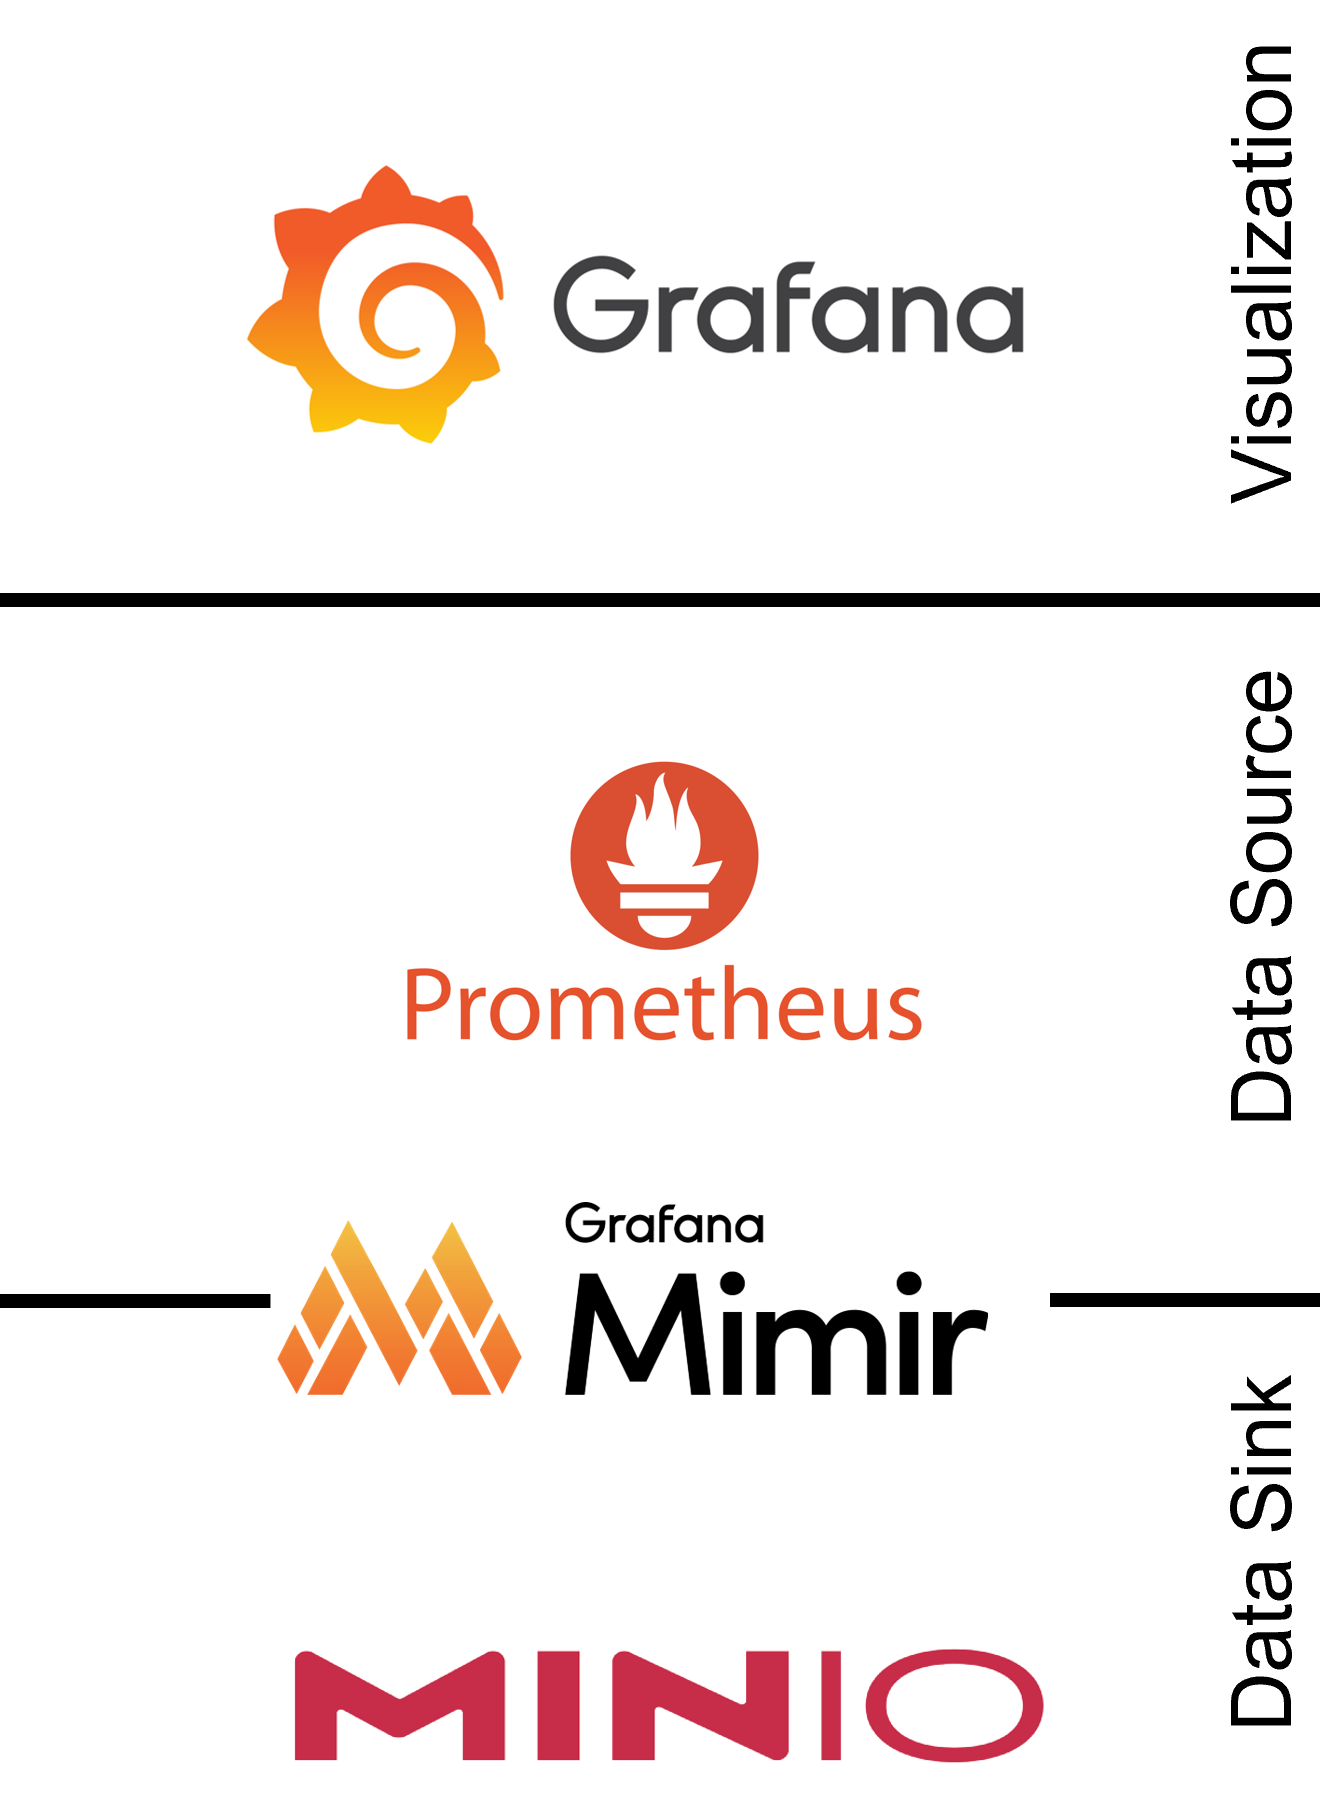
\includegraphics[width=0.4\textwidth]{figures/spmonitor_tech_stack.png}
% 	\caption{SPMonitor Technology Stack}
% 	\label{fig:spmonitor_tech_stack}
% \end{figure}

% From these three options, Prometheus together with Grafana, Mimir, and MinIO was chosen for SPMonitor.
% Unlike OpenTelemetry, Prometheus provides easy integration with its data sink and visualization tool as
% they were built to work together. OpenTelemetry on the other hand is a standalone solution meant to enhance
% other tools which do not collect metrics themselves. The TICK stack provides the same integration benefit compared
% to OpenTelemetry. The decision between Prometheus and the TICK stack is not as straightforward.
% Both fulfill all requirements, offer extensibility options through plugins for different data sources
% and pre-built visualizations, and they are both open-source projects which can be freely used.
% One difference between them is that there exists a provider solution for managing Grafana with Crossplane.
% This does not seem to exist for the TICK stack. Crossplane will be used to provision and operate the cloud
% services of \Gls{DLAKaApp} and SPMonitor. Therefore Grafana and Prometheus are chosen for SPMonitor as they offer tools
% for integrating them with Crossplane compared to the TICK stack. The final selection of tools can be seen in Figure \ref{fig:spmonitor_tech_stack}.

\subsection{SPS Architecture}

% TODO: Do

\begin{figure}[h]
	\centering
	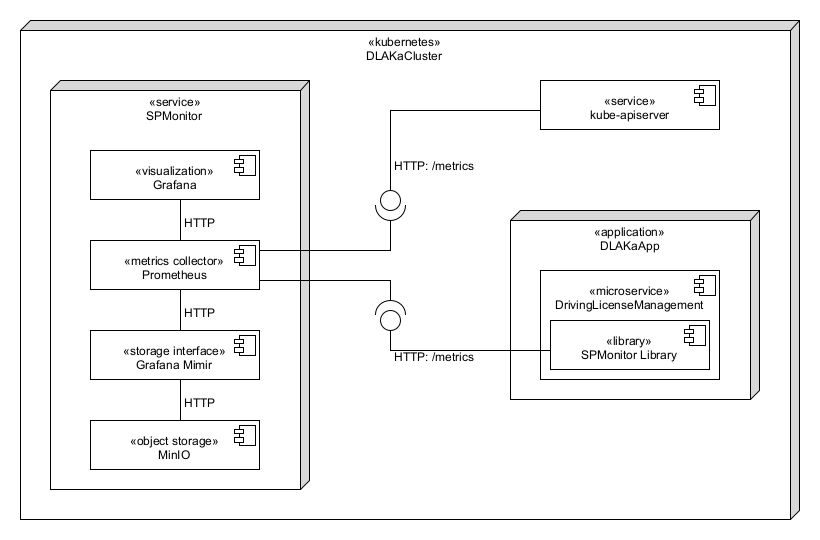
\includegraphics[width=\textwidth]{figures/sps_spmonitor.png}
	\caption{SystemPlusSoftware for SPMonitor}
	\label{fig:sps_spmonitor}
\end{figure}

\section{Implementation and Deployment}
\label{sec:impl_and_deployment}

% TODO: Add Helm to Design

% Implementation and Deployment:
% - Implementation:
% 	- SPMonitor Library and integration into AM-DLM
% - Deployment:
% 	- Separate Helm Charts
% 		- Prometheus
% 			- service discovery
% 		- Grafana
% 			- preloading dashboards
% 		- Minio
% 		- Custom Mimir Chart
% 	- Combining the charts into a single chart

SPMonitor was designed to be run as a single Helm Chart.
The first step to achieving this was to create separate Helm Charts for the individual
services which would later be combined into a single Helm Chart.

Because SPMonitor was designed to be run as a Helm Chart,
there was no implementation for most of the services of SPMonitor
as all services, except Mimir, already provide suitable Helm Charts which only
need to be configured. For the first iteration of SPMonitor, a separate Helm Chart
was created for each service. These would then later be combined into a single
Helm Chart.

The Helm Chart for Prometheus was developed first as it is the central service of SPMonitor.

\cite{PRO-HELM}

\cite{GRA-HELM}

\cite{MIM-IMG}

\cite{MIN-HELM}